% ACC 2027 / PaperPlaza official class. ieeeconf.cls MUST sit in the project
% root next to this file - Overleaf does not search subfolders for .cls.
\documentclass[letterpaper, 10 pt, conference]{ieeeconf}

\IEEEoverridecommandlockouts   % required before \thanks in ieeeconf
\overrideIEEEmargins           % required to meet the ACC printer margins

\usepackage{amsmath,amssymb,bm}
\let\proof\relax
\let\endproof\relax
\usepackage{amsthm} % for theorem/proof environments
\usepackage{booktabs,array,cite}
\usepackage{graphicx}
\usepackage{float} % enables [H] (and helps with class restrictions on lone [h])
\usepackage[hidelinks]{hyperref}
% Figures live under figures/..., so keep that on the graphics path.
\graphicspath{{figures/}{figures/disturbance/}{../experiments/nengo_nef_replication_2026-08-29/results/plots/}}

% [v6] TikZ support for the architecture figures.
\usepackage{tikz}
\usepackage{verbatim}
\usetikzlibrary{arrows.meta,positioning,fit,backgrounds,calc}
% Architecture drawing helpers live in architectures/tikz/.
% Shared TikZ style for all architecture figures. Grayscale-safe.
\tikzset{
  blk/.style   ={draw,rounded corners=2pt,align=center,font=\footnotesize,
                 minimum height=8mm,inner sep=3pt,fill=white},
  clas/.style  ={blk,fill=black!4},
  neuro/.style ={blk,fill=black!12,very thick},
  plant/.style ={blk,fill=black!20},
  meas/.style  ={blk,dashed},
  sum/.style   ={draw,circle,inner sep=0pt,minimum size=4.5mm,font=\scriptsize},
  sig/.style   ={-{Latex[length=2mm]},thick},
  sigd/.style  ={-{Latex[length=2mm]},thick,dashed},
  lbl/.style   ={font=\scriptsize,inner sep=1.5pt,fill=white},
  grp/.style   ={draw,dashed,rounded corners=3pt,inner sep=6pt},
  note/.style   ={font=\scriptsize\itshape,align=left},
}


\newcommand{\R}{\mathbb R}
\newcommand{\T}{^{\mathsf T}}
\newcommand{\sat}{\operatorname{sat}}
\newcommand{\sgnp}{\operatorname{sgn}_{+}}

\newtheorem{proposition}{Proposition}

% [v7] Title now names the mechanism and the learning, and claims the
% controlled study rather than architectural novelty.
\title{\LARGE \bf Online Prescribed Error Sensivity Decoder Learning in Neuromorphic Residual UAV Attitude Control}

% ACC/PaperPlaza template author format (ieeeconf.cls does not support IEEEtran blocks).
\author{Gandhi Contreras$^{1}$, Steven Sandoval$^{1}$, and Luis Rodolfo Garcia Carrillo$^{2}$%
\thanks{$^{1}$New Mexico State University (NMSU), Las Cruces, NM, USA.}%
\thanks{$^{2}$ Space Vehicles Directorate, Air Force Research Laboratory (AFRL), Kirtland Air Force Base (KAFB), Albuquerque, NM 87108.
    Email: {\tt\small luis\_rodolfo.garcia\_carrillo@afrl.af.mil}}%
}

\usepackage{etoolbox}
\apptocmd{\thebibliography}{\itemsep=-1pt\relax}{}{}
% [v11] Layout only: tighter float separation and fuller float pages. Template fonts unchanged.
\setlength{\textfloatsep}{6pt plus 2pt minus 2pt}
\setlength{\floatsep}{5pt plus 2pt minus 2pt}
\setlength{\intextsep}{5pt plus 2pt minus 2pt}
\setlength{\dbltextfloatsep}{6pt plus 2pt minus 2pt}
\setlength{\dblfloatsep}{5pt plus 2pt minus 2pt}
\setlength{\abovecaptionskip}{3pt}
\setlength{\belowcaptionskip}{0pt}
\renewcommand{\topfraction}{0.92}
\renewcommand{\bottomfraction}{0.5}
\renewcommand{\textfraction}{0.08}
\renewcommand{\floatpagefraction}{0.8}
\renewcommand{\dbltopfraction}{0.92}
\renewcommand{\dblfloatpagefraction}{0.8}
\begin{document}
% IEEE reference practice: lists of more than six authors print as "et al."
\bstctlcite{IEEEexample:BSTcontrol}
\maketitle

% NOTE: The official ACC/PaperPlaza template typically suppresses page numbers for
% submission. Uncomment the next two lines only for internal review.
% \pagestyle{plain}
% \thispagestyle{plain}


\begin{abstract}
Quadrotor attitude controllers must track time-varying references while respecting coupled rotor-force limits under uncertainty, noise, and disturbances. We propose an online neuromorphic residual in which six continuous membrane-gate (CMG) units generate temporal features and eighteen decoder weights adapt online via prescribed error sensitivity (PES).
%
The residual adds a bounded correction to a saturated quaternion PD controller before rotor-force allocation: it enforces explicit authority bounds, exactly recovers the baseline when disabled, and uses a saturation-aware output gate that prevents opposing an axis already at its torque limit.
%
Against a bandwidth-tuned PD with desired-rate feedforward (PD+ff), the gated residual reduces geometric-mean attitude error by $37.3\%$ (X2) and $22.4\%$ (CF2) noise-free, and reduces burst-phase error under repeated torque disturbances by $14\%$ and $6\%$. With sensor noise, it preserves $4$--$11\%$ gains on multi-axis missions and is neutral or slightly negative at the noise floor.
Under the same tuned PD+ff baseline, an Izhikevich basis increases geometric-mean error by $18.9\%$ (X2) and $5.4\%$ (CF2) at about twice the realized CMG effort.
The residual can be paired directly with LQR, sliding-mode, and model-predictive baselines, and in simulation improves tracking across the tested families and platforms.
\end{abstract}


%%%%%%%%%%%%%%%%%%%%%%%%%%%%%%%%%%%%
\section{Introduction}
%%%%%%%%%%%%%%%%%%%%%%%%%%%%%%%%%%%%
Classical feedback provides an interpretable stabilizing backbone for quadrotor attitude control, but unmodeled effects and abrupt disturbances can leave structured tracking errors that are hard to remove without retuning or increasing actuator demand. Residual control adds an adaptive correction around an existing feedback law while preserving its plant and actuator interface. \looseness = -1

Residual learning has been paired with classical controllers in robotics \cite{johannink2019}, including geometric $\mathcal L_1$ quadrotor augmentation \cite{wu2025l1quad}. Related brain-inspired UAS controllers combine model-based feedback with learned terms \cite{rubioscola2023limbic,rubioscola2021mambo}. Neuromorphic platforms support stateful adaptive corrections through the Neural Engineering Framework and online decoder learning \cite{eliasmith2004neuraleng,bekolay2014nengo}, commonly using the local prescribed-error-sensitivity (PES) rule \cite{voelker2015pes}. NEF-based spiking controllers have been designed for quadrotor dynamics with fixed, not online-adapted, weights \cite{garciaalcantara2024snnuas}. More recently, self-tuning spiking PID control has been demonstrated for a quadrotor \cite{olivares2026selftuning}. However, continuous membrane--gate features for actuator-aware quaternion residual control, and the separate roles of neuron dynamics and decoder learning, remain insufficiently characterized.
%
This gap is especially relevant for real-time execution. The coupled membrane--gate (CMG) dynamics are continuous and integrated with a fixed-step update (Sec.~\ref{sec:main}), avoiding the step-size collapse and numerical drift concerns that can arise with stiff event-driven spiking models. Learning uses the local PES rule, so online adaptation requires only instantaneous error and activity and avoids the memory and replay overhead of backpropagation-through-time \cite{voelker2015pes,bellec2020eprop}.

We study a bounded online residual controller for quaternion UAV attitude tracking under individual rotor-force limits. A saturated quaternion PD(+ff) baseline supplies the nominal torque request, and a neuromorphic CMG--PES module provides a compact stateful realization of the residual correction via six continuous membrane--gate (CMG) units and an eighteen-parameter prescribed error sensitivity (PES) decoder.
The contributions are: (i) a bounded residual interface for attitude-torque augmentation with explicit authority limits and exact baseline-command recovery at zero residual authority (Fig.~\ref{fig:arch}); (ii) a saturation-aware gate that prevents the residual from opposing an axis already at the prescribed torque limit; (iii) a fully specified CMG--PES realization with paired nonnegative activity, bounded readout, and online local adaptation; and (iv) a two-platform, five-mission simulation study against fixed and bandwidth-tuned baselines (PD+ff primary), including measurement-noise and repeated-disturbance tests, and portability across conventional controller families without per-mission retuning.

%A neuron-family comparison (Sec.~\ref{sec:family}) shows that under the same protocol an Izhikevich basis needs about ten times CMG's effort while performing no better, isolating decoder adaptation, not persistent activity alone, as the mechanism.

The remainder of this paper is organized as follows. Section~\ref{sec:problem} formulates the problem. Section~\ref{sec:main} presents the proposed controller and the bounded-interface result, with discussion in Section~\ref{sec:discussion} and proofs in Section~\ref{sec:proofs}. Section~\ref{sec:application} reports the numerical experiments, and Section~\ref{sec:conclusion} concludes and outlines future work.

%%%%%%%%%%%%%%%%%%%%%%%%%%%%%%%%%%%%%%%%%%%%%%%%%%
\section{Problem Formulation}
\label{sec:problem}
%%%%%%%%%%%%%%%%%%%%%%%%%%%%%%%%%%%%%%%%%%%%%%%%%%
We seek to reduce shortest-path attitude-tracking error for a prescribed reference $q_d(t)$ while respecting coupled actuator limits induced by individual rotor-force bounds. A baseline attitude law (e.g., PD+ff, LQR, SMC, MPC/NMPC) produces a requested body torque $\bm u_0$; the proposed neuromorphic residual may add a bounded correction to form $\bm u$, after which the same rotor allocator and per-rotor saturation produce the realized actuator torque $\bm\tau_{\rm act}$. The residual is constrained to preserve a fixed componentwise authority bound and to recover the baseline exactly when its authority is set to zero; no closed-loop stability claim is assumed from these interface properties.

\subsection{Process, State, and Tracking Error}

Let $Q\in\mathbb S^3$ be the scalar-first Hamilton quaternion mapping body to
inertial coordinates, and let $\bm\omega$ be the body angular velocity. The
rotational dynamics are \cite{schaub2018amss}
\begin{align}
 \dot Q&=\tfrac12 Q\otimes[0,\bm\omega\T]\T,\\
 \bm J\dot{\bm\omega}&=\bm\tau_{\rm act}+\bm\tau_{\rm p}
       +\bm\tau_{\rm d}-\bm\omega\times(\bm J\bm\omega).
 \label{eq:plant}
\end{align}
where $\bm J\succ0$ is the body-frame inertia and
$\bm\tau_{\rm act}$ is the body torque realized by the actuators.
The terms $\bm\tau_{\rm p}$ and $\bm\tau_{\rm d}$ denote modeled
passive and externally applied disturbance torques, respectively.
The controller produces a requested body torque $\bm u$, which is
mapped to $\bm\tau_{\rm act}$ through the rotor allocation and force
constraints defined in Sec.~II-B.

Using the corresponding passive quaternion $q=Q^{-1}$ \cite{diebel2006quaternion}, define
%\cite{diebel2006quaternion}
\begin{equation}
 \dot q=-\tfrac12[0,\bm\omega\T]\T\otimes q.
 \label{eq:passive}
\end{equation}
The desired attitude $q_d$ uses the same convention. Define the attitude error
\begin{align}
 q_e&=q_d\otimes q^{-1}=[q_{e,0},\bm q_{e,v}\T]\T,\\
 \bm e_q&=\sgnp(q_{e,0})\bm q_{e,v},\qquad \sgnp(0)=1,\\
 \theta_q&=2\operatorname{atan2}(\|\bm q_{e,v}\|_2,|q_{e,0}|)
             \in[0,\pi].
 \label{eq:theta}
\end{align}
The metric $\theta_q$ is invariant to the quaternion sign. No continuous feedback globally stabilizes rigid-body attitude \cite{chaturvedi2011rigid}; global formulations require, for example, hybrid switching \cite{mayhew2011hybrid} or geometric-algebra methods \cite{rubioscola2026ga}. We use the shortest-path branch away from the $180^\circ$ sign boundary.

For a desired-frame rate $\bm\omega_d$ satisfying the corresponding passive kinematics, differentiation gives
\begin{align}
 \dot q_e&=\tfrac12q_e\otimes[0,\bm\omega_e\T]\T,\\
 \bm\omega_e&=\bm\omega-R(q_e)\T\bm\omega_d,\qquad
 \dot q_{e,0}=-\tfrac12\bm q_{e,v}\T\bm\omega_e.
 \label{eq:errkin}
\end{align}
These relations follow directly from the attitude-error quaternion kinematics. \looseness=-1
%These are kinematic identities; no convergence claim is implied.\looseness=-1

Let $\bm J\succ0$ denote the body-frame inertia \cite{schaub2018amss}. If principal moments $\bm j_{\rm p}$ are given in a rotated principal-axis frame, then
\begin{equation}
 \bm J=R_{BI}\operatorname{diag}(\bm j_{\rm p})R_{BI}\T,
 \label{eq:inertiaframe}
\end{equation}
with $R_{BI}$ the principal-to-body rotation. Controller gains use the reported principal moments in their given ordering, $\bm j_{\rm tune}$ (Table~\ref{tab:models}).

\subsection{Actuation and Sensing}
%
For rotor positions $\bm p_i$ in body coordinates, parallel $+z$ thrust
axes, and signed reaction coefficients $\kappa_i$, define
\begin{equation}
 B=\begin{bmatrix}
 1&1&1&1\\p_{1,y}&p_{2,y}&p_{3,y}&p_{4,y}\\
 -p_{1,x}&-p_{2,x}&-p_{3,x}&-p_{4,x}\\
 \kappa_1&\kappa_2&\kappa_3&\kappa_4
 \end{bmatrix}.
 \label{eq:allocationmatrix}
\end{equation}
The signs follow $\bm p_i\times[0,0,f_i]\T$ and the actuator's local reaction torque $\kappa_i f_i$ \cite{garciacarrillo2013quad}. Here $B$ maps rotor thrusts to total thrust and body torque; $\kappa_i$ has units of meters, not angular velocity. Given a commanded collective thrust $T$ and body-torque command $\bm u$, the corresponding inverse-allocation with per-rotor saturation model is
\begin{equation}
 \begin{aligned}
 \bm f_{\rm req}&=B^{-1}[T,\bm u\T]\T,\\
 \bm f_{\rm act}&=\sat_{[\bm0,\bm f_{\max}]}(\bm f_{\rm req}),\\
 [T_{\rm act},\bm\tau_{\rm act}\T]\T&=B\bm f_{\rm act}.
 \end{aligned}
 \label{eq:mixer}
\end{equation}
Here $\bm u=\bm u_0$ for PD; the CMG path in Section~\ref{sec:main}
modifies that requested torque before the same allocation and saturation.
The operator $\sat_{[\bm a,\bm b]}(\cdot)$ denotes componentwise saturation to the interval $[a_i,b_i]$, i.e.,
$\bigl(\sat_{[\bm a,\bm b]}(\bm x)\bigr)_i=\min\{\max\{x_i,a_i\},b_i\}$.
Each $f_i$ is a commanded force in newtons, not a rotor-speed command.
Exact wrench realization requires $B^{-1}[T,\bm u\T]\T\in[\bm0,\bm f_{\max}]$; for four
rotors $B$ is square and invertible, so $B^{-1}=B^{\dagger}$.
A componentwise torque box is not generally contained in this
collective-dependent feasible set. This work uses inverse allocation followed by componentwise saturation,
not an optimization-based allocator \cite{monteiro2016allocation}.\looseness=-1

Collective thrust remains classical, with $z_d=1$ m:
\begin{equation}
 T=\sat_{[0,2.5Mg]}
 \left(\frac{M[g+6(z_d-z)-4\dot z]}{\max(R(Q)_{33},0.35)}\right).
 \label{eq:collective}
\end{equation}

Here $g$ is the gravitational acceleration. The height loop reads altitude and vertical velocity; the denominator compensates tilt.
The guard $0.35$ limits tilt compensation to about $\arccos(0.35)\approx69.5^\circ$, and the upper bound does
not supersede individual rotor limits. The residual has no direct collective
output but can affect height through attitude, tilt compensation, and
saturation.
The feedback variables used by the attitude and height loops are $q$, $\bm\omega$, $z$, and $\dot z$. In the nominal simulations they are read directly from the model; Sec.~\ref{sec:noise} perturbs the measured attitude and rate before they enter the controller. No additional state or plant output is provided to the residual path.

\begin{figure*}[!th]
    \centering
    \resizebox{0.90\textwidth}{!}{% Fig. 1 -- CMG-PES residual control architecture (picture only; no preamble).
% For ACC2027.tex: \input{architectures/fig1_architecture_body.tex} inside figure* (e.g. \resizebox{0.95\textwidth}{!}{...}).
% Requires arch_style.tex, \sat, \sgnp, \T, \bm and the TikZ libraries arrows.meta, positioning, fit, backgrounds, calc.
\tikzset{
  blk/.append style={font=\footnotesize,inner sep=3.5pt},
  neuro/.append style={fill=blue!10,draw=black!65,thick},          % neuromorphic residual path: light blue
  gatek/.style={blk,fill=orange!12,draw=orange!70!black,thick},     % saturation-aware gate: orange
  plant/.append style={fill=blue!22,draw=blue!75!black,very thick}, % MuJoCo plant: strong blue
  online/.style={draw=blue!60!black,thin,dash pattern=on 1.2pt off 1.2pt,rounded corners=4pt},
}
\begin{tikzpicture}[x=1cm,y=1cm]
  % ------------------------------------------------------------------ classical loop (top row)
  \node[clas] (ref) at (2.6,1.75) {\textbf{Mission reference}\quad $q_{d,k},\ \bm\omega_{d,k}$};
  \node[clas] (pd) at (2.6,0) {\textbf{Quaternion error and PD+ff}\\[1pt]
      $q_{e,k}=q_{d,k}\otimes q_k^{-1}$\\
      $\bm e_{q,k}=\sgnp(q_{e,0,k})\,\bm q_{e,v,k}$\\
      $\bm u_{0,k}=\sat_{\bm\ell}\big(-K_q\bm e_{q,k}-K_\omega(\bm\omega_k-\bm\omega_{d,k})\big)$};
  \node[clas] (add) at (9.9,0) {\textbf{Bounded torque addition}\\[1pt]
      $\tilde{\bm\delta}_k=\beta\,\bm\ell\odot\tilde{\bm s}_k$\\
      $\bm u_k=\sat_{\bm\ell}(\bm u_{0,k}+\tilde{\bm\delta}_k)$};
  \node[clas] (alloc) at (14.6,0) {\textbf{Rotor allocation}\\\textbf{and force limits}\\[1pt]
      $\bm f_{{\rm req},k}=B^{-1}[T_k,\bm u_k\T]\T$\\
      $\bm f_{{\rm act},k}=\sat_{[\bm 0,\bm f_{\max}]}(\bm f_{{\rm req},k})$};
  \node[plant] (plant) at (19.2,0) {\textbf{MuJoCo plant}\\\textbf{X2 / CF2}\\[1pt]
      $[T_{{\rm act},k},\bm\tau_{{\rm act},k}\T]\T=B\bm f_{{\rm act},k}$\\rigid-body dynamics};
  \node[clas] (height) at (19.2,-2.85) {\textbf{Height controller}\\[1pt]
      $T_k=\sat_{[0,\,2.5Mg]}\big(\pi_z(z_k,\dot z_k,R_{33,k})\big)$\\$z_d=1$\,m};

  \draw[sig] (ref) -- (pd);
  \draw[sig] (pd) -- node[lbl,above,pos=0.62]{$\bm u_{0,k}$} coordinate[pos=0.22] (u0tap) (add);
  \draw[sig] (add) -- node[lbl,above]{$\bm u_k$} (alloc);
  \draw[sig] (alloc) -- node[lbl,above]{$\bm f_{{\rm act},k}$} (plant);
  \draw[sig] (plant) -- node[lbl,right]{$z_k,\dot z_k,R_{33,k}$} (height);
  \draw[sig] ($(height.north west)+(0.35,0)$) |- node[lbl,pos=0.3,left]{$T_k$} ($(alloc.east)+(0,-0.62)$);

  % ------------------------------------------------------------------ CMG-PES residual path
  \node[neuro] (enc) at (3.25,-3.55) {\textbf{Paired currents}\\[1pt]
      $\bar{\bm u}_k=\bm u_{0,k}\oslash\bm\ell$\\
      $\bm I^\pm_k=I_b\bm 1+I_g\max(\pm\bar{\bm u}_k,\bm 0)$};
  \node[neuro] (cmg) at (7.75,-3.55) {\textbf{Six CMG units}\\[1pt]
      $(\bm v_k,\bm r_k;\bm I_k)\mapsto(\bm v_k^+,\bm r_k^+)$\\
      $\bm a_k=\sat_{[0,1]}(G\bm r_k^+)$};
  \node[neuro] (dec) at (12.05,-3.55) {\textbf{Decoder and output bound}\\[1pt]
      $\bm s_k=\sat_{[-1,1]}(W_k\bm a_k)$};
  \node[gatek] (gate) at (11.7,-1.80) {\textbf{Saturation-aware gate}\\[1pt]
      $\tilde s_{k,i}=0$ if $|u_{0,k,i}|\ge\ell_i$ and $s_{k,i}u_{0,k,i}<0$\\
      else $\tilde s_{k,i}=s_{k,i}$ \ (output only; PES unmasked)};
  \node[neuro] (tgt) at (3.4,-6.45) {\textbf{PES teaching target}\\[1pt]
      $\bm y^*_k=\sat_{[-1,1]}(-k_e\bm e_{q,k}-k_\omega^*\bm\omega_k)$};
  \node[neuro] (pes) at (9.15,-6.45) {\textbf{PES update, leak, and projection}\\[1pt]
      $\bm\varepsilon_k=\bm y^*_k-\bm s_k$\\
      $W_{k+1}=\Pi_{\mathcal W}\big[(1-\lambda_W)W_k+\eta\,\bm\varepsilon_k\bm a_k\T\big]$};
  \node[neuro] (mem) at (14.3,-6.45) {\textbf{Decoder memory}\\[1pt]one-step delay\\$W_0=[I_3,\,-I_3]$};

  % residual signals
  \draw[sig] (pd.south-|enc) -- node[lbl,right]{$\bm u_{0,k}$} (enc.north);
  \draw[sig] (enc) -- node[lbl,above]{$\bm I_k$} (cmg);
  \draw[sig] (cmg) -- node[lbl,above]{$\bm a_k$} coordinate[pos=0.35] (atap) (dec);
  \fill (atap) circle (1.4pt);
  \draw[sig] (atap) -- node[lbl,right,pos=0.5]{$\bm a_k$} (atap|-pes.north);
  \draw[sig] (dec.north-|gate.south) -- node[lbl,right]{$\bm s_k$} (gate.south);
  \draw[sig] (gate.north-|add) -- node[lbl,right]{$\tilde{\bm s}_k$} (add.south);
  \draw[sigd] (u0tap) |- node[lbl,pos=0.78,above]{$\bm u_{0,k}$: load test} (gate.west);
  \fill (u0tap) circle (1.4pt);
  \coordinate (sx) at ($(pes.north east)+(-0.45,0)$);
  \draw[sig] (sx|-dec.south) -- node[lbl,right,pos=0.45]{$\bm s_k$ (pre-gate)} (sx);
  \draw[sig] (tgt) -- node[lbl,above]{$\bm y^*_k$} (pes);
  \draw[sig] (pes) -- node[lbl,above]{$W_{k+1}$} (mem);
  \draw[sig] (mem.east) -- ++(0.55,0) |- node[lbl,pos=0.25,right]{$W_k$} (dec.east);
  \draw[sig] (mem.south) -- ++(0,-0.55) -| node[lbl,pos=0.25,below]{$W_k$} (pes.south);

  % PES teaching signal: the attitude error computed in the PD block and the measured rate
  \coordinate (eqx) at ($(pd.south west)+(0.25,0)$);
  \fill (eqx) circle (1.4pt);
  \draw[sig] (eqx) -- node[lbl,fill=white,rotate=90,pos=0.42,above]{$\bm e_{q,k}$ (error block), $\bm\omega_k$ (measured)} (eqx|-tgt.west) -- (tgt.west);

  % feedback: measured attitude and rate
  \coordinate (fbx) at ($(height.east)+(0.35,0)$);
  \draw[sig] (plant.east) -| (fbx|-0,-8.45) -| node[lbl,pos=0.06,above]{measured attitude and rate:\ $q_k=Q_k^{-1},\ \bm\omega_k$} (-0.75,0) -- (pd.west);

  % neuromorphic online part: thin fine-dashed boundary (the gate is a classical interface, kept outside)
  \coordinate (loopbot) at ($(mem.south)+(0,-0.95)$);
  \begin{scope}[on background layer]
    \node[online,inner sep=6pt,fit=(enc)(cmg)(dec)(tgt)(pes)(mem)(loopbot)] (rp) {};
  \end{scope}
  \node[note,anchor=south west,text=blue!60!black] at ($(rp.south west)+(0.12,0.08)$) {neuromorphic, learns online (CMG--PES)};
\end{tikzpicture}
}
    \caption{CMG-PES neuromorphic residual control architecture with online PES decoder learning. The classical feedback, collective-thrust, allocation, and plant interfaces are retained; only the bounded decoder output augments the requested attitude torque, after the saturation-aware gate \eqref{eq:gate} masks any component that opposes a saturated baseline axis.}
    \label{fig:arch}
\end{figure*}

\subsection{Quaternion PD Baselines and Control Objective}

The quaternion PD baseline is
\begin{align}
 \bm k_q&=2\bm j_{\rm tune}\odot\bm\omega_n^2,\qquad
 \bm k_\omega=2\zeta\bm j_{\rm tune}\odot\bm\omega_n,\\
 \bm u_0&=\sat_{\bm\ell}(-\bm k_q\odot\bm e_q-\bm k_\omega\odot\bm\omega),
 \label{eq:pd}
\end{align}
with $\bm\omega_n=(4,4,3.5)\T$ rad/s and $\zeta=0.95$. The torque box is
$\mathcal U=\prod_{i=1}^3[-\ell_i,\ell_i]$, where
$\ell_i=\max(j_{{\rm tune},i}\nu_i,10^{-6}\ \mathrm{N\,m})$ and
$\bm\nu=(12,12,10)\T$ rad/s$^2$; this component bound on the commanded torque does not, by itself, guarantee that the resulting command is feasible under the individual rotor limits.

Since the derivative term in \eqref{eq:pd} damps absolute body rate,
we also consider a PD baseline with desired-rate feedforward (PD+ff),
obtained by replacing $\bm\omega$ with the rate-tracking error
$\bm\omega-\bm\omega_d$:
\begin{equation}
 \bm u_0^{\rm ff}=\sat_{\bm\ell}\bigl(-\bm k_q\odot\bm e_q-\bm k_\omega\odot(\bm\omega-\bm\omega_d)\bigr),
 \label{eq:pdff}
\end{equation}

The design objective is therefore: given the classical torque request $\bm u_0$, construct an online residual correction that reduces $\theta_q$ over time-varying missions while (i) retaining the same attitude and angular rate measurements, collective-thrust loop, rotor allocator, and actuator limits, (ii) imposing an explicit componentwise bound on the deviation from $\bm u_0$, and (iii) recovering the requested baseline exactly when residual authority is set to zero. These implementation properties don't guarantee closed-loop stability.


%%%%%%%%%%%%%%%%%%%%%%%%%%%%%%%%%%%%%%%%%%%%%%%%%%%%%%%%%%%%%%%%%
\section{Main Result: Online Neuromorphic Residual Controller}
\label{sec:main}
%%%%%%%%%%%%%%%%%%%%%%%%%%%%%%%%%%%%%%%%%%%%%%%%%%%%%%%%%%%%%%%%%
The proposed control framework decouples the adaptive internal dynamics from a bounded residual correction added to the baseline torque command. By setting the residual authority $\beta = 0$, the controller recovers the exact baseline torque request. Figure~\ref{fig:arch} details the overall signal flow.


\subsection{CMG Temporal Features}

For $m$ torque channels and $2m$ units, normalize the saturated baseline and
form positive/negative current pairs:
\begin{equation}
 \begin{aligned}
 \bar{\bm u}&=\bm u_0\oslash\bm\ell,\\
 \bm I^{\pm}&=I_b\bm1+I_g\max(\pm\bar{\bm u},\bm0),\\
 \bm I&=[(\bm I^+)\T,(\bm I^-)\T]\T.
 \end{aligned}
 \label{eq:encoding}
\end{equation}
Each unit has a dimensionless membrane state $v_j$ and gate $r_j$:
\begin{align}
 \dot r_j&=[\sigma(\alpha_h(v_j-v_{\rm th}+\gamma r_j))-r_j]/\tau_r,\\
 \dot v_j&=-(v_j-v_{\rm rest})/\tau+I_j/\tau-c_j(v_j-v_{\rm reset}),\\
 c_j&=(g_0+\chi g_1|I_j|)r_j^2,\qquad \chi\in\{0,1\}.
 \label{eq:cmg}
\end{align}
Here $\sigma(x)=(1+e^{-x})^{-1}$ denotes the logistic sigmoid, which bounds the gate activation to $(0,1)$.

\begin{figure}[t]
\centering
\resizebox{0.86\columnwidth}{!}{% Fig. 2 -- coupling topology of one CMG unit (picture only; no preamble). Light-blue neuromorphic blocks, as in Fig. 1.
% For ACC2027.tex: \input{architectures/fig2_cmg_unit_body.tex} inside a figure (fits one IEEE column).
% Requires arch_style.tex and \sat. The state equations stay in the text; the figure shows which variable acts on which.
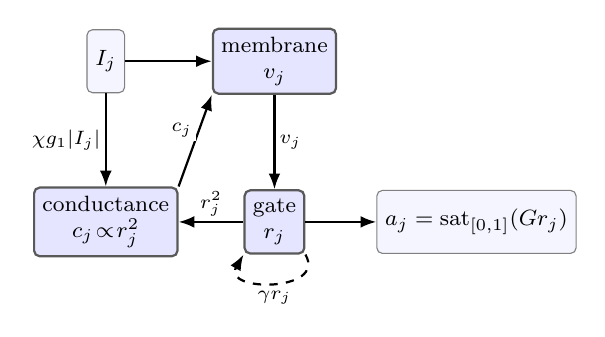
\begin{tikzpicture}[node distance=6mm and 9mm,font=\footnotesize,
    nb/.style={blk,fill=blue!10,draw=black!65,thick},       % neuromorphic state blocks (light blue)
    nbl/.style={blk,fill=blue!4,draw=black!50}]             % input/output and auxiliary blocks (lighter)
  \node[nbl]                        (I) {$I_j$};
  \node[nb,right=11mm of I]         (v) {membrane\\$v_j$};
  \node[nb,below=12mm of v]         (r) {gate\\$r_j$};
  \node[nb] at (I|-r)               (c) {conductance\\$c_j\!\propto\! r_j^{2}$};
  \node[nbl,right=9mm of r]         (a) {$a_j=\sat_{[0,1]}(G r_j)$};

  \draw[sig] (I) -- (v);
  \draw[sig] (v) -- node[lbl,right]{$v_j$} (r);
  \draw[sig] (r) -- node[lbl,above]{$r_j^{2}$} (c);
  \draw[sig] (c.north east) -- node[lbl,above left=-1pt]{$c_j$} (v.south west);
  \draw[sig] (I) -- node[lbl,left]{$\chi g_1|I_j|$} (c);
  \draw[sig] (r) -- (a);
  \draw[sigd] (r.south east) to[out=-60,in=-120,looseness=1.8] node[lbl,below=1pt]{$\gamma r_j$} (r.south west);
\end{tikzpicture}}
\caption{Coupling topology of one CMG unit, cf.~(\ref{eq:cmg}). The membrane sets
 the gate target; the gate acts back twice, shifting its own threshold through
 $\gamma$ and shunting the membrane through $c_j\propto r_j^2$ ($\chi=1$ makes
 that shunt input dependent). The dynamics are continuous: no spike, no reset,
 and only $a_j$ leaves the unit.}
\label{fig:cmgunit}
\end{figure}


%
The gate dynamics in \eqref{eq:cmg} are a first-order relaxation: the bounded sigmoid output $\sigma(\alpha_h(v_j-v_{\rm th}+\gamma r_j))\in(0,1)$ provides an instantaneous reference level that depends on membrane voltage and is modulated by feedback from the current gate state. The gate state $r_j$ then relaxes toward that time-varying reference with time constant $\tau_r$. In parallel, $r_j$ modulates membrane conductance through $c_j\propto r_j^2$ (Fig.~\ref{fig:cmgunit}), so both states participate even though the decoder reads only the gate-derived activity. The model has no threshold-triggered reset or spike event; $v_{\rm reset}$ is a reversal level in a continuous conductance term. The gains $g_0,g_1$ have the units needed to make $c_j$ a rate.

The actual integration is sequential, not exponential Euler for both
states. From the old states compute
\begin{align}
 b_{j,k}&=\sigma\!\left(\sat_{[-60,60]}
       [\alpha_h(v_{j,k}-v_{\rm th}+\gamma r_{j,k})]\right),\\
 r_{j,k}^{+}&=\sat_{[0,1]}
       [r_{j,k}+(h/\tau_r)(b_{j,k}-r_{j,k})].
 \label{eq:gate_step}
\end{align}
Then evaluate $c_{j,k}=(g_0+\chi g_1|I_{j,k}|)(r_{j,k}^{+})^2$,
$\lambda_{j,k}=\tau^{-1}+c_{j,k}$, and
$d_{j,k}=(v_{\rm rest}+I_{j,k})/\tau+c_{j,k}v_{\rm reset}$. By holding $\lambda_{j,k}$ and $d_{j,k}$ constant over one integration interval $h$, the membrane equation is affine in $v_j$ and integrates exactly to
\begin{equation}
 v_{j,k}^{+}=e^{-\lambda_{j,k}h}v_{j,k}
       +(1-e^{-\lambda_{j,k}h})d_{j,k}/\lambda_{j,k}.
 \label{eq:mem_step}
\end{equation}
The coefficients are recomputed at the start of the next numerical step; \eqref{eq:mem_step} is therefore an exact per-step exponential update under that within-step hold, guaranteeing a non-divergent numerical update within the interval. However, this local step formulation does not establish closed-loop stability for the fully coupled, nonlinear UAV dynamics and adaptive controller. Assign $(v_{j,k+1},r_{j,k+1})=(v_{j,k}^{+},r_{j,k}^{+})$.
The exponential-Euler step $r_{j,k}^{+}=e^{-h/\tau_r}r_{j,k}+(1-e^{-h/\tau_r})b_{j,k}$ is
convex for every $h>0$ without saturation, and changes only the weight on $r_{j,k}$
($0.905$ vs.\ $0.9$ at $h/\tau_r=0.1$); all simulation benchmarks in Section~VI use \eqref{eq:gate_step}.



\subsection{PES Decoder Adaptation and Bounded Residual}

The within-step activity, initial decoder, and saturated readout are
\begin{equation}
 \begin{aligned}
 \bm a_k&=\sat_{[0,1]}(G\bm r_k^+),\qquad W_0=[I_m,-I_m],\\
 \bm s_k&=\sat_{[-1,1]}(W_k\bm a_k).
 \end{aligned}
 \label{eq:readout}
\end{equation}
The initial readout matrix $W_0=[I_3,-I_3]$ implements paired-channel
subtraction ($a^+-a^-$), recovering signed directional information from
a nonnegative activity basis; state memory can delay sign reversal
following a command reversal. With $G=10^5$, the nonnegative activity
$a_j=\sat_{1}(G r_j^+)$ reaches its upper bound of $1$
when $r_j^+\ge10^{-5}$. Since $r_j^+\ge0$, the symmetric
saturation $\sat_{1}$ acts here over $[0,1]$. Thus, the activity
gain $G$ determines how strongly $r_j^+$ is amplified before the
readout decoder and how quickly the resulting activity saturates. The teaching target and local update are
\begin{align}
 \bm y_k^*&=\sat_{[-1,1]}(-k_e\bm e_{q,k}-k_\omega^*\bm\omega_k),\\
 \bm\varepsilon_k&=\bm y_k^*-\bm s_k,\\
 W_{k+1}&=\Pi_{\mathcal W}
       [W_k+\eta\bm\varepsilon_k\bm a_k\T-\lambda_W W_k].
 \label{eq:pes}
\end{align}
Here $\mathcal W=[-W_{\max},W_{\max}]^{m\times2m}$. The coefficients $\eta$ and $\lambda_W$ are per-step (so changing $h$ changes the effective learning dynamics). PES is a local error-driven update toward the prescribed target $\bm y_k^*$; it does not differentiate through the plant or claim to minimize a closed-loop cost.

Using $W_k$ before the update, the requested command is
\begin{equation}
 \bm u_k=\sat_{\bm\ell}(\bm u_{0,k}+\beta\bm\ell\odot\bm s_k),\quad
 \bm\delta_k=\bm u_k-\bm u_{0,k},\quad 0\le\beta\le1.
 \label{eq:residual}
\end{equation}
For three-axis UAV attitude control ($m=3$), the network consists of
six CMG units and eighteen decoder weights.

\paragraph{Saturation-aware gate}
At $|u_{0,k,i}|=\ell_i$ the residual acts one-sidedly: a component with the sign of $u_{0,k,i}$ is saturated away, whereas an opposing one removes up to $\beta\ell_i$ of authority exactly when the loop needs all of it. The gated residual therefore replaces $\bm s_k$ in \eqref{eq:residual} by
\begin{equation}
 \tilde s_{k,i}=\begin{cases}0,&|u_{0,k,i}|\ge\ell_i\ \text{and}\ s_{k,i}u_{0,k,i}<0,\\ s_{k,i},&\text{otherwise,}\end{cases}
 \label{eq:gate}
\end{equation}
and leaves the PES update \eqref{eq:pes} untouched. Since $|\tilde{s}_{k,i}| \le |s_{k,i}|$, the gate cannot increase
 the residual magnitude and introduces no additional tuning parameter.
 The resulting interface bounds and baseline-recovery property are
 established formally in Proposition~\ref{prop:bounded}.

\begin{proposition}[Bounded residual interface and baseline recovery]\label{prop:bounded}
Assume the nonnegative CMG parameters of Table~\ref{tab:parameters}, $r_{j,0}\in[0,1]$, $0<h\le\tau_r$, $W_0\in\mathcal W$, and $\bm u_{0,k}\in\mathcal U$. Then: (i) every gate remains in $[0,1]$ and each membrane iterate remains in the convex hull of its initial value, $v_{\rm reset}$, and $[v_{\rm rest}+I_b,v_{\rm rest}+I_b+I_g]$; (ii) the projected update keeps $W_k\in\mathcal W$; and (iii) $\bm u_k\in\mathcal U$ with $|\delta_{k,i}|\le\beta\ell_i$. If $\beta=0$, the requested baseline command is recovered at every step, and the same allocator at the same state and collective thrust produces the same actuator output.
\end{proposition}

\textit{Remark 1 (Interpretation of Bounds):}
The bounds in (i)--(ii) keep the adaptive CMG/PES states within their
prescribed operational domains. In contrast, property (iii) is directly
exposed to the closed-loop system: it bounds the residual torque
modification and guarantees exact recovery of the baseline command when
$\beta=0$, independently of the learned internal state.

%%%%%%%%%%%%%%%%%%%%%%%%%%%%%%%%%%%%%%%%%%%%%%%%%%%%%%%%%%%%%%%%%
\section{Discussion of the Main Result}
\label{sec:discussion}
%%%%%%%%%%%%%%%%%%%%%%%%%%%%%%%%%%%%%%%%%%%%%%%%%%%%%%%%%%%%%%%%%
Proposition~\ref{prop:bounded} establishes implementation bounds that hold for every $\beta\in[0,1]$, hence for the gated controller actually used in the experiments. Its scope is deliberately limited: it is an operational interface bound, not an input-to-state stability certificate, and bounded internal states, weights, and requested torque do not establish state safety, rotor headroom, closed-loop stability, or improved tracking. Rotor-force saturation can also couple requested torque components, so the componentwise residual bound is not a trajectory-to-trajectory robustness certificate.

A restricted fixed-feature PES contraction observation is summarized in Sec.~\ref{sec:ablation} (Remark~\ref{rem:pes}) and is used only to interpret activity-limited learning behavior; it is not a closed-loop convergence result.

%%%%%%%%%%%%%%%%%%%%%%%%%%%%%%%%%%%%%%%%%%%%%%%%%%%%%%%%%%%%%%%%%
\section{Proofs}
\label{sec:proofs}
%%%%%%%%%%%%%%%%%%%%%%%%%%%%%%%%%%%%%%%%%%%%%%%%%%%%%%%%%%%%%%%%%
\begin{proof}[Proof of Proposition~\ref{prop:bounded}]
For the gate update, $b_{j,k}\in[0,1]$ and $0<h\le\tau_r$ make the unsaturated Euler step a convex combination of $r_{j,k}$ and $b_{j,k}$; the componentwise saturation in \eqref{eq:gate_step} therefore preserves $r_{j,k}\in[0,1]$. Since $I_j\in[I_b,I_b+I_g]$ and $c_j\ge0$, $d_j/\lambda_j$ is a convex combination of $v_{\rm rest}+I_j$ and $v_{\rm reset}$. Equation~\eqref{eq:mem_step} is a convex combination of $v_{j,k}$ and $d_j/\lambda_j$, so induction gives the membrane bound. Projection in \eqref{eq:pes} gives $W_k\in\mathcal W$. Finally, the outer saturation in \eqref{eq:residual} gives $\bm u_k\in\mathcal U$; componentwise nonexpansiveness and $\sat_{\ell_i}(u_{0,k,i})=u_{0,k,i}$ imply $|\delta_{k,i}|\le|\beta\ell_i s_{k,i}|\le\beta\ell_i$. Setting $\beta=0$ gives $\bm u_k=\bm u_{0,k}$, after which the common allocator produces the same actuator output at the same state and collective thrust.
\end{proof}



%%%%%%%%%%%%%%%%%%%%%%%%%%%%%%%%%%%%%%%%%%%%%%%%%%%%%%%%%%%%%%%%%
\section{Application and Examples}
\label{sec:application}
%%%%%%%%%%%%%%%%%%%%%%%%%%%%%%%%%%%%%%%%%%%%%%%%%%%%%%%%%%%%%%%%%
\subsection{Platforms, Missions, and Metrics}
% [v13] Vehicle-photo strip removed from the flow to meet the page limit: it carried no technical
% content and was never referenced in the text.  Restore by deleting the \iffalse/\fi pair.
\begin{figure*}[t]
\centering
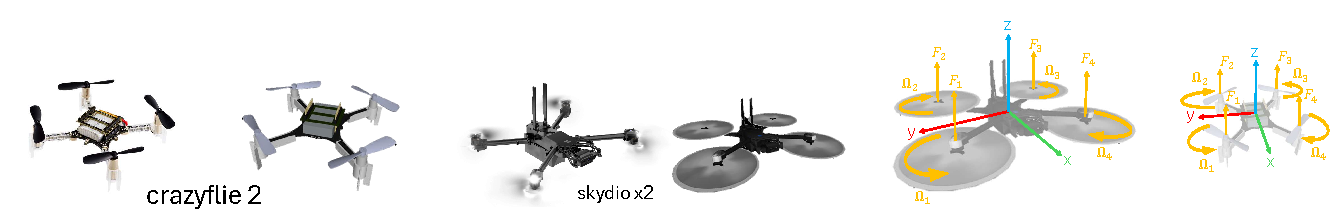
\includegraphics[width=\textwidth]{figures/01_mujoco_missions/fig2_drones_only.pdf}
\caption{Vehicles and simulation models. Left: CF2 hardware and MuJoCo model. Center: X2 hardware and MuJoCo model. Right: both geometries at relative scale.}
\label{fig:models}
\end{figure*}

Let $\mathcal{B}=\{\bm b_x,\bm b_y,\bm b_z\}$ denote the body-fixed axis triad and $\mathcal{P}=\{\bm p_1,\bm p_2,\bm p_3\}$ the principal-inertia triad. The angular velocity, commanded and realized torques, and rotor geometry are expressed in $\mathcal{B}$. If the principal moments $\bm j_{\rm p}$ are specified in $\mathcal{P}$, the body-frame inertia is
\begin{equation*}
    \bm J=R_{BP}\operatorname{diag}(\bm j_{\rm p})R_{BP}\T,
\end{equation*}
where $R_{BP}$ maps principal-frame coordinates into the body frame (cf.~\eqref{eq:inertiaframe}).

We evaluate in MuJoCo rigid-body simulation with site-applied actuator wrenches
\cite{todorov2012mujoco}, using two Menagerie-derived multirotors (CF2, X2; Fig.~\ref{fig:models})
\cite{menagerieModels}. The attitude loop commands body torque and the height loop
collective thrust. For CF2 we expose four rotor-force channels and use the inverse allocator with per-rotor saturation \eqref{eq:mixer}. Table~\ref{tab:models} lists simulation parameters and
spec-context values. For CF2 the per-rotor force limit is raised to $1.5\times$ the Menagerie model value ($0.0875\to0.13125$ N, Table~\ref{tab:models}) so that the tuned baseline is not permanently rotor-saturated; this is a simulation design choice, not a claim about Crazyflie hardware. X2 uses its model limit unchanged. Both models omit motor/RPM/battery states and validated rotor
aerodynamics; feedback uses \texttt{qpos}/\texttt{qvel}, with noise only in Sec.~\ref{sec:noise}. The controllers run in Nengo~4.1.0 (a custom \texttt{NeuronType} with direct current injection; its teaching graph adds a one-step latency), and a direct NumPy realization agrees to $2.013\times10^{-6}$ relative mean error over ten cases, which is tested numerical agreement, not formal equivalence.
%
\begin{table}[t]
\centering
\caption{Model/interface parameters (top) and canonical CMG--PES settings (bottom). Neural quantities are normalized model variables; learning coefficients are per step.}
\label{tab:models}\label{tab:parameters}
\setlength{\tabcolsep}{3pt}\renewcommand{\arraystretch}{0.93}
\footnotesize
\begin{tabular}{@{}p{0.40\linewidth}p{0.27\linewidth}p{0.25\linewidth}@{}}
\toprule
Parameter & CF2 rotor model & X2 model\\
\midrule
Mass $M$ (kg) & $0.027$ & $1.325$\\
Rotor $|p_x|,|p_y|$ (m) & $0.0325,0.0325$ & $0.14,0.18$\\
Reaction magnitude $|\kappa_i|$ (m) & $0.005$ & $0.0201$\\
Rotor force limit (N) & $.0875\to.13125$ & $13$\\
$\bm j_{\rm tune}$ ($10^{-5}$ kg\,m$^2$) & $(2.3951,\allowbreak2.3951,\allowbreak3.2347)$ & ---\\
$\bm j_{\rm tune}$ ($10^{-2}$ kg\,m$^2$) & --- & $(6.0711,\allowbreak3.6468,\allowbreak2.5412)$\\
Rigid-body integrator & RK4 & Euler\\
\bottomrule
\end{tabular}
\par\medskip
\footnotesize\setlength{\tabcolsep}{3pt}
\begin{tabular}{@{}ll@{\hspace{6pt}}ll@{}}
\toprule
CMG--PES & Value & & Value\\\midrule
$h$, duration & $0.0005$ s, $45$ s & $\alpha_h,\gamma,g_0,g_1$ & $50,2,120,30$\\
$\tau,\tau_r$ & $0.05$ s, $0.005$ s & $I_b,I_g,G$ & $0.75,1.25,10^5$\\
$v_{\rm rest},v_{\rm reset},v_{\rm th}$ & $0,0,1$ & $\beta_{\rm X2},\beta_{\rm CF2};\eta$ & $.5,.2;\,8\times10^{-4}$\\
$v_{j,0},r_{j,0},\chi$ & $0,0,1$ & $\lambda_W,W_{\max},k_e,k^*_\omega$ & $10^{-6},6,8,0$\\
\bottomrule
\end{tabular}
\end{table}
%
\begin{figure}[!t]
\centering
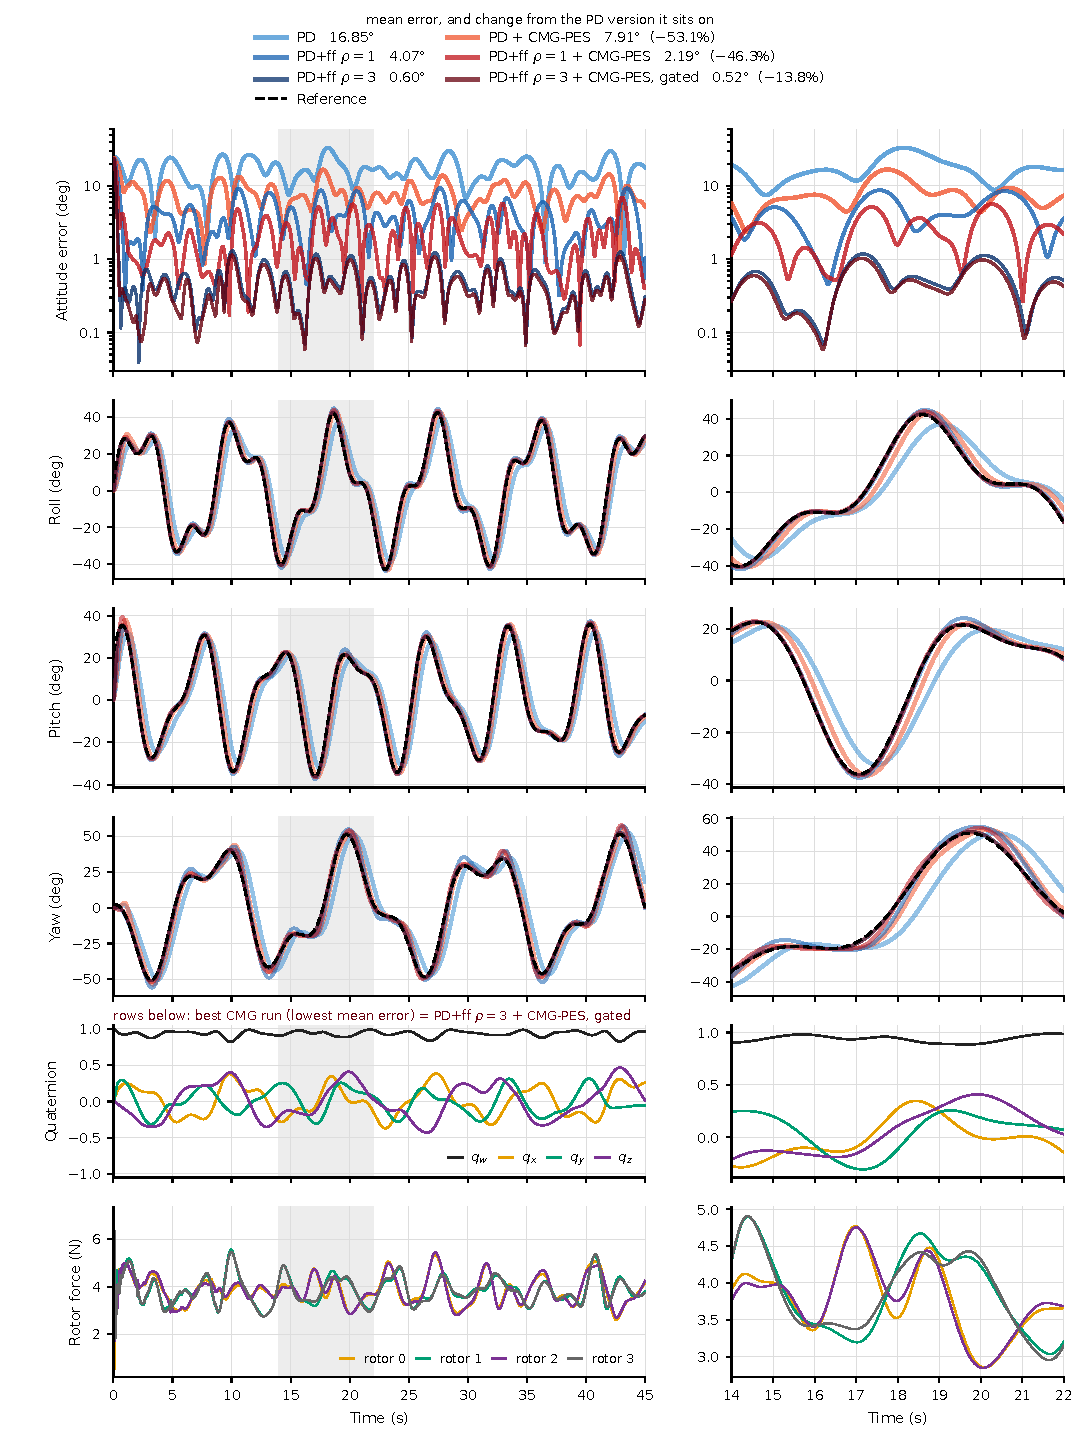
\includegraphics[width=\linewidth]{figures/10_hard45/x2_hard45_ladder.pdf}
\caption{X2 Hard45 tracking (45\,s) across the baseline ladder. Blue: PD baselines (light$\to$dark: fixed PD, PD+ff $\rho{=}1$, tuned PD+ff $\rho{=}3$). Red: CMG--PES paired with each baseline (matched shading); the $\rho{=}3$ pair is gated ($\beta{=}.5$).}
\label{fig:tracking}
\end{figure}
%
Code, model files, and run archives accompany the submission as a reproducibility package.\footnote{\url{https://github.com/gandhico/online-pes-neuromorphic-residual-control}}

CF2 body axes are principal. For X2 the geometry-derived inertia is
$\bm J=10^{-2}[3.66517,0,-.21000;\allowbreak\,0,2.54117,0;\allowbreak\,-.21000,0,6.05280]$\,kg\,m$^2$;
torque limits use $\bm j_{\rm tune}$.

Each PD/CMG pair shares initial state, reference, duration, allocator, model, and timestep. The residual authority is $\beta=.5$ on X2 and $\beta=.2$ on CF2, with the saturation-aware gate \eqref{eq:gate} in the $\rho=3$ results. Without the gate, a predeclared sweep over $\beta\in\{.5,.2,.1,.05,.02\}$ (lowest five-mission geometric-mean error ratio among settings with every error below $1$ rad and saturation fraction below $.5$) admits only $\beta=.05$ on CF2, because larger values diverge on Hardstep (Sec.~\ref{sec:failure}). The gate lifts that restriction noise-free, but not under measurement noise (Sec.~\ref{sec:noise}), where $\beta=.2$ is the largest sweep value that stayed safe: it was chosen on two development seeds and confirmed on $13$ held-out ones. The $\rho=1$ and fixed-PD rows of Table~\ref{tab:all} are ungated. The primary campaign is deterministic (no injected disturbances or noise), one run per cell, with learning active throughout.

The primary tracking metric is the time-averaged scalar orientation error $\bar{\theta}_q=\frac{1}{N}\sum_{k=1}^{N}\theta_{q,k}$, reported in milliradians (mrad), where $1\,\mathrm{mrad}=10^{-3}\,\mathrm{rad}\approx0.0573^\circ$. We also report the relative reduction $100(\bar\theta_{q,\rm PD}-\bar\theta_{q,\rm CMG})/\bar\theta_{q,\rm PD}$.

For readability, the reference missions are specified below as Euler-angle
triples and converted to the desired quaternion $q_d(t)$; attitude-error
computation and feedback control remain quaternion based.
Reference Euler triples (rad): Roll $(0.25\sin0.7t,0,0)$; Full3 $0.5\sin(t+(0,\pi/2,\pi)\T)$; Hard45
$(0.55\sin0.75t+0.20\sin(2.10t+0.40),\allowbreak\;0.45\sin(0.95t+\pi/3)+0.18\sin1.75t,\allowbreak\;0.65\sin(0.55t+\pi)+0.25\sin(1.35t+0.20))$;
Hardstep: $0$ for 1 s then 2-s cycles through $(.75,-.45,.55)$, $(-.65,.55,-.70)$, $(.50,.50,.90)$, $(-.80,-.35,.20)$; Yaw360 $(0,0,2\pi(3\xi^2-2\xi^3))$, $\xi=t/45$. Hover, whose nominal error is near zero, is used only for the disturbance test.



\subsection{Comparison with Classical Baselines}
\label{sec:baselines}

The fixed PD law in \eqref{eq:pd} damps absolute rate, so moving references can contain a velocity-lag contribution. We therefore use the desired-rate feedforward law~\eqref{eq:pdff} as the stronger baseline comparison and introduce a dimensionless bandwidth scaling factor $\rho>0$, which scales the nominal natural frequency according to $\bm\omega_n\mapsto\rho\bm\omega_n$. We sweep $\rho\in[0.75,8]$, where $\rho=1$ recovers the nominal closed-loop bandwidth. The best mission-mean occurs at $\rho=3$ on both airframes; CF2 becomes rotor-limited beyond approximately $\rho=4$. This bandwidth-tuned PD+feedforward controller is the primary baseline.\looseness=-1

At $\rho=3$, the gated CMG--PES residual ($\beta=.5$ on X2, $.2$ on CF2) reduces the geometric-mean error from $4.54\times10^{-3}$ to $2.85\times10^{-3}$ rad on X2 ($37.3\%$) and from $3.77\times10^{-3}$ to $2.92\times10^{-3}$ rad on CF2 ($22.4\%$). It improves Roll, Full3, Hard45 (Fig.~\ref{fig:tracking}), and Yaw360 on both vehicles; Hardstep is the only mission that does not improve (Sec.~\ref{sec:failure}). The geometric mean is dominated by Roll and Yaw360, where PD+ff errors are already below $0.6$ mrad; on Full3 and Hard45 the reductions are $12$--$14\%$ (X2) and $5$--$7\%$ (CF2). Without the gate, CF2 admits only $\beta=.05$ and the reduction is $6.5\%$ (Table~\ref{tab:all}, ungated row). Against the original fixed PD law (Table~\ref{tab:all}, which also gives the $\rho=1$ ladder), the residual lowers mean quaternion-angle error in all ten nominal cases by $17.3$--$60.6\%$, so the apparent margin shrinks as the classical baseline is strengthened.

\paragraph{Portability across control families} The residual attaches unmodified to four families beyond PD+ff, by replacing only the nominal law $\bm u_0$ in \eqref{eq:residual}: LQR, sliding-mode control (SMC), unconstrained model-predictive control (MPC), and nonlinear MPC (NMPC), each at the same bandwidth scaling and gate settings, plus a PID variant with rotor-level conditional-integration anti-windup. The gated residual improves the geometric mean for every family on both platforms, with no exceptions: LQR $31.1\%$/$22.4\%$ (X2/CF2), PID+ff $36.7\%$/$22.4\%$, SMC $43.8\%$/$26.6\%$, MPC $33.4\%$/$22.7\%$, and NMPC $31.9\%$/$21.7\%$. SMC gains the most specifically on Hardstep, where its own baseline is weaker; LQR and MPC each show a large \emph{baseline} error on CF2 Hardstep from the linear-quadratic family's small torque margin there, unrelated to the residual. This is an interface-portability result, not a claim that the residual is tuned for each family; a full per-family study is future work.

\begin{table*}[!t]
\caption{Mean $q$-error ($10^{-3}$\,rad, 45\,s). $\Delta$: reduction over the block baseline [\%]. Effort: RMS residual / per-axis bound. Closing column: geometric mean (error rows), arithmetic mean (effort rows).}
\label{tab:all}\centering\scriptsize\setlength{\tabcolsep}{3.0pt}\renewcommand{\arraystretch}{0.93}
\begin{tabular}{@{}lrrrrrr@{\hspace{7pt}}rrrrrr@{}}
\toprule
&\multicolumn{6}{c@{\hspace{7pt}}}{Skydio X2}&\multicolumn{6}{c}{Crazyflie~2}\\
\cmidrule(lr){2-7}\cmidrule(l){8-13}
 & Roll & Full3 & Hard45 & Hardstep$^\dagger$ & Yaw360 & \emph{geo} & Roll & Full3 & Hard45 & Hardstep$^\dagger$ & Yaw360 & \emph{geo}\\
\midrule
\multicolumn{13}{@{}l}{\textit{Primary baseline: PD + rate feedforward, $\rho=3$ (bandwidth-tuned)}}\\[1pt]
PD+ff & 0.34 & 10.09 & 10.54 & 265.91 & 0.20 & \emph{4.54} & 0.56 & 7.06 & 8.65 & 262.59 & 0.084 & \emph{3.77}\\
\;+CMG--PES, gated & 0.074 & 8.83 & 9.08 & 271.35 & 0.12 & \emph{2.85} & 0.23 & 6.67 & 8.02 & 263.19 & 0.067 & \emph{2.92}\\
\;\;$\Delta$ [\%] & 78.4 & 12.4 & 13.8 & -2.0 & 41.8 & \emph{37.3} & 59.9 & 5.4 & 7.3 & -0.2 & 20.3 & \emph{22.4}\\
\;+CMG--PES, ungated$^\ddagger$ & 0.074 & 8.83 & 9.08 & 311.07 & 0.12 & \emph{2.93} & 0.43 & 6.96 & 8.50 & 265.93 & 0.079 & \emph{3.52}\\
\;\;$\Delta$ [\%] & 78.4 & 12.4 & 13.8 & -17.0 & 41.8 & \emph{35.6} & 22.9 & 1.3 & 1.8 & -1.3 & 5.6 & \emph{6.5}\\
\;\;$\Delta$, realistic noise [\%] & -4.2 & 11.3 & 10.8 & -2.6 & -5.3 & \emph{2.3} & -0.4 & 3.9 & 4.0 & -0.3 & -2.2 & \emph{1.0}\\
\;\;$\Delta$, moderate noise [\%] & -1.4 & 11.9 & 11.2 & -2.4 & -3.9 & \emph{3.3} & 2.2 & 4.2 & 4.2 & -0.2 & -2.0 & \emph{1.7}\\
\midrule
\multicolumn{13}{@{}l}{\textit{Baseline ladder: PD + rate feedforward, $\rho=1$}}\\[1pt]
PD+ff & 2.98 & 72.10 & 71.02 & 454.77 & 1.78 & \emph{26.19} & 4.91 & 42.72 & 53.18 & 425.93 & 0.74 & \emph{20.39}\\
\;+CMG--PES & 0.61 & 32.81 & 38.17 & 359.16 & 0.60 & \emph{11.04} & 0.97 & 20.29 & 28.23 & 347.68 & 0.25 & \emph{8.65}\\
\;\;$\Delta$ [\%] & 79.5 & 54.5 & 46.3 & 21.0 & 66.4 & \emph{57.8} & 80.2 & 52.5 & 46.9 & 18.4 & 66.4 & \emph{57.6}\\
\midrule
\multicolumn{13}{@{}l}{\textit{Original fixed PD baseline, $\bm\omega_n=(4,4,3.5)$ rad/s}}\\[1pt]
PD & 50.56 & 303.28 & 294.08 & 454.53 & 75.86 & \emph{173.12} & 51.34 & 288.38 & 285.45 & 426.18 & 75.81 & \emph{168.68}\\
\;+CMG--PES & 41.79 & 131.75 & 138.01 & 359.35 & 29.90 & \emph{96.02} & 42.44 & 126.48 & 132.32 & 347.89 & 29.87 & \emph{94.11}\\
\;\;$\Delta$ [\%] & 17.4 & 56.6 & 53.1 & 20.9 & 60.6 & \emph{44.5} & 17.3 & 56.1 & 53.6 & 18.4 & 60.6 & \emph{44.2}\\
\;\;$\Delta$, fixed decoder [\%] & 1.9 & 9.7 & 10.3 & 0.5 & 0.1 & \emph{4.6} & 3.3 & 4.5 & 6.8 & 0.4 & 0.1 & \emph{3.1}\\
\midrule
\multicolumn{13}{@{}l}{\textit{Strongest rival basis (Izhikevich): reduction and realized effort}}\\[1pt]
\;\;$\Delta$, Izhikevich--PES, $\rho=3$ [\%] & -48.0 & 5.8 & 4.5 & -1.1 & -76.3 & \emph{-18.9} & 0.7 & 1.3 & 0.8 & -0.5 & -33.3 & \emph{-5.4}\\
\;\;$\Delta$, Izhikevich--PES, fixed PD [\%] & 39.6 & 37.5 & 32.2 & 6.6 & 46.6 & \emph{33.8} & 33.7 & 38.9 & 32.2 & diverges$^\S$ & 41.5 & \emph{--}\\
\;\;$\Delta$, Izhikevich fixed dec., fixed PD [\%] & 4.6 & 4.9 & 4.6 & 0.7 & 0.2 & \emph{3.0} & 5.6 & 5.8 & 4.0 & -2.2 & -2.2 & \emph{2.3}\\
\;\;effort, CMG--PES, $\rho=3$ & 0.003 & 0.023 & 0.023 & 0.109 & 0.001 & \emph{0.032} & 0.005 & 0.010 & 0.012 & 0.049 & $<$0.001 & \emph{0.015}\\
\;\;effort, Izhikevich--PES, $\rho=3$ & 0.053 & 0.051 & 0.053 & 0.106 & 0.052 & \emph{0.063} & 0.012 & 0.021 & 0.021 & 0.047 & 0.012 & \emph{0.023}\\
\bottomrule
\end{tabular}
\par\smallskip
\begin{minipage}{\textwidth}\scriptsize
LIF/ALIF/LIFRate stay within $0.1\%$ of fixed PD outside Hardstep. $\rho=3$ rows are gated \eqref{eq:gate} with $\beta=.5$ (X2), $.2$ (CF2); $^\ddagger$ungated, $\beta=.5$, $.05$ (the $\rho=1$ and fixed-PD rows are ungated). $^\dagger$Hardstep commands $63$--$111^\circ$ steps every $2$\,s; $97$--$99\%$ of its mean error is slew (Sec.~\ref{sec:failure}). $^\S$CF2 Hardstep under the fixed-PD baseline sustains near-$180^\circ$ tracking loss ($2.45$\,rad mean, $t{=}3$--$44$\,s); excluded from the geometric mean rather than averaged in.
\end{minipage}
\end{table*}


%We use the desired-rate feedforward baseline \eqref{eq:pdff} (Sec.~II-C) as the stronger comparison and sweep $\bm\omega_n\mapsto\rho\bm\omega_n$ over $\rho\in[0.75,8]$. The best mission-mean occurs at $\rho=3$ on both airframes; CF2 becomes rotor-limited beyond approximately $\rho=4$. This bandwidth-tuned PD+feedforward controller is the primary baseline.\looseness=-1

%At $\rho=3$, the gated CMG--PES residual ($\beta=.5$ on X2, $.2$ on CF2) reduces the geometric-mean error from $4.54\times10^{-3}$ to $2.85\times10^{-3}$ rad on X2 ($37.3\%$) and from $3.77\times10^{-3}$ to $2.92\times10^{-3}$ rad on CF2 ($22.4\%$). It improves Roll, Full3, Hard45 (Fig.~\ref{fig:tracking}), and Yaw360 on both vehicles; Hardstep is the only mission that does not improve (Sec.~\ref{sec:failure}). The geometric mean is dominated by Roll and Yaw360, where PD+ff errors are already below $0.6$ mrad; on Full3 and Hard45 the reductions are $12$--$14\%$ (X2) and $5$--$7\%$ (CF2). Without the gate, CF2 admits only $\beta=.05$ and the reduction is $6.5\%$ (Table~\ref{tab:all}, ungated row). Against the original fixed PD law (Table~\ref{tab:all}, which also gives the $\rho=1$ ladder), the residual lowers mean quaternion-angle error in all ten nominal cases by $17.3$--$60.6\%$, so the apparent margin shrinks as the classical baseline is strengthened.

\subsection{Mechanism Ablation}
\label{sec:ablation}

The architecture separates intrinsic conductance modulation ($\chi$), decoder adaptation ($W_k$), and residual authority ($\beta\bm\ell$), which affect the CMG dynamics, learned activity-to-output mapping, and maximum residual torque, respectively. This separation allows the effects of the internal dynamics, online learning, and residual authority to be examined separately.

We ablate decoder adaptation (PES) and conductance modulation ($\chi$). With decoder mode held fixed, toggling $\chi$ (retaining the base shunt $g_0r_j^2$) is numerically indistinguishable. The reason is structural: $\chi$ enters only through $c_j\propto r_j^2$, which is $2\times10^{-9}\,\mathrm{s}^{-1}$ at rest against a leak of $\tau^{-1}=20\,\mathrm{s}^{-1}$; after a gate latches (below) it only moves the membrane fixed point ($0.107\to0.092$ at $I_j=I_b$), which the saturated activity hides from the readout.
\textit{Remark 2 (Fixed-feature PES contraction):}\label{rem:pes}
If the teaching target and a nonzero activity $\bm a$ are fixed, decoder leak is zero, and readout saturation and projection remain inactive, then the PES error contracts as
\begin{equation}
 \bm\varepsilon_{k+1}=(1-\eta\|\bm a\|_2^2)\bm\varepsilon_k,
 \label{eq:contraction}
\end{equation}
so a nonzero initial error contracts to zero when $0<\eta\|\bm a\|_2^2<2$. This constant-feature calculation \cite{voelker2015pes} is used only to interpret activity-limited learning behavior; changing targets, loss of excitation, saturation, leakage, and plant dynamics prevent direct application as a closed-loop convergence statement.

\emph{Fixed versus adaptive decoder.} Holding $W_k=W_0$ keeps CMG dynamics but limits the readout to the paired difference $\bm a^+-\bm a^-$, and yields only modest reductions (Table~\ref{tab:all}).

\emph{Gate/activity regime.} At $I_j=I_b$, $v_j\approx0.75<v_{\rm th}$ and $r_j\approx\sigma(-12.5)\approx3.7\times10^{-6}$, i.e., a small but nonzero logistic tail. Once $r_j\ge1/2$, Proposition~\ref{prop:bounded} implies $b_{j,k}\ge1/2$ in \eqref{eq:gate_step}, so opened gates latch; with $G=10^5$ the resting activity is $a_j\approx0.37$ and latched units saturate at $a_j=1$.

When activity is effectively constant ($\bm a_k\approx\bar{\bm a}$) and projection is inactive, the PES update reduces to the recursion for $\bm z_k=W_k\bar{\bm a}$
\begin{equation}
 \bm z_{k+1}=(1-\lambda_W)\bm z_k
 +\eta\|\bar{\bm a}\|^2[\bm y_k^*-\sat_{[-1,1]}(\bm z_k)],
 \label{eq:constantbasis}
\end{equation}
a leaky first-order filter of the teaching target (Remark~\ref{rem:pes}), i.e., lagged proportional action with corner $9.60$ rad/s. Hard45's highest instantaneous frequency is $2.1$ rad/s \cite{sandoval2018instantaneous}, below that corner. These ablations indicate that decoder adaptation is the dominant lever in the tested regime: the CMG dynamics provide a bounded graded/latched basis on which PES shapes the correction.

%We ablate decoder adaptation (PES) and conductance modulation ($\chi$). With decoder mode held fixed, toggling $\chi$ (retaining the base shunt $g_0r_j^2$) is numerically indistinguishable. The reason is structural: $\chi$ enters only through $c_j\propto r_j^2$, which is $2\times10^{-9}\,\mathrm{s}^{-1}$ at rest against a leak of $\tau^{-1}=20\,\mathrm{s}^{-1}$; after a gate latches (below) it only moves the membrane fixed point ($0.107\to0.092$ at $I_j=I_b$), which the saturated activity hides from the readout.

%\emph{Fixed versus adaptive decoder.} Holding $W_k=W_0$ keeps CMG dynamics but limits the readout to the paired difference $\bm a^+-\bm a^-$, and yields reductions of only $4.6\%$ (X2) and $3.1\%$ (CF2) geometric mean (Table~\ref{tab:all}).

%A matched-effort non-neural residual (e.g., a filtered-P or leaky-integrator correction with comparable authority) was not run in this campaign. Equation~\eqref{eq:constantbasis} shows that under near-constant activity the PES readout is itself such a filter, so the tested regime is one where a linear residual could in principle match the decoder's tracking. The contribution here is therefore not the filter shape but the bounded, gate-compatible, baseline-recoverable interface through which it acts; a matched-effort comparison is left to future work.

%\emph{Gate/activity regime.} At $I_j=I_b$, $v_j\approx0.75<v_{\rm th}$ and $r_j\approx\sigma(-12.5)\approx3.7\times10^{-6}$, i.e., a small but nonzero logistic tail. Once $r_j\ge1/2$, Proposition~\ref{prop:bounded} implies $b_{j,k}\ge1/2$ in \eqref{eq:gate_step}, so opened gates latch; with $G=10^5$ the resting activity is $a_j\approx0.37$ and latched units saturate at $a_j=1$.

%When activity is effectively constant ($\bm a_k\approx\bar{\bm a}$) and projection is inactive, the PES update reduces to the recursion for $\bm z_k=W_k\bar{\bm a}$

%\begin{equation}
% \bm z_{k+1}=(1-\lambda_W)\bm z_k
% +\eta\|\bar{\bm a}\|^2[\bm y_k^*-%\clip_{[-1,1]}(\bm z_k)],
% \label{eq:constantbasis}
%\end{equation}

%a leaky first-order filter of the teaching target (Proposition~\ref{prop:pes}), i.e., lagged proportional action with corner $9.60$ rad/s. Hard45's highest instantaneous frequency is $2.1$ rad/s \cite{sandoval2018instantaneous}, below that corner. These ablations indicate that decoder adaptation is the dominant lever in the tested regime: the CMG dynamics provide a bounded graded/latched basis on which PES shapes the correction.

\subsection{Neuron-Family Comparison}
\label{sec:family}

The Nengo benchmark isolates the basis choice, holding one actuator interface fixed across two models, five missions, and eleven controllers (PD plus fixed/PES variants of CMG, LIF, ALIF, Izhikevich \cite{izhikevich2003}, and LIFRate); only the neuron dynamics and native-state-to-activity map differ. Across the full matrix (figure omitted) two patterns hold. First, PES is the dominant lever in every family: fixed decoders rarely match their PES counterparts, extending Sec.~\ref{sec:ablation} to every basis. Second, persistent activity is necessary but not sufficient. Remark~\ref{rem:pes} explains the flat rows: a sparsely active basis starves the update. In the corrected $\rho=3$ runs, LIF, ALIF and LIFRate have mission-mean activity occupancy (activity $>10^{-6}$) of $3.2$--$4.4\%$, whereas CMG (resting at $a_j\approx0.37$) and Izhikevich are active in ${\ge}99.9\%$.

Izhikevich--PES leads on the fixed-PD baseline (Table~\ref{tab:all}, last block) but not on the tuned one: under the primary protocol it is positive but below CMG on Full3 and Hard45 ($+5.8/+4.5\%$ vs.\ CMG's $+12.4/+13.8\%$ on X2), while its residual sits on a $\pm\beta\ell$ rail in only $0$--$1.7\%$ of samples, similar to CMG's own low rail occupancy, its effort still averages about twice CMG's because it stays near $0.05$--$0.06$ regardless of mission rather than tracking the baseline error as CMG's does. On Roll and Yaw360, where the baseline is already near the noise floor, the residual raises the geometric-mean error to $1.19\times$ (X2) and $1.05\times$ (CF2) the baseline's; CMG's own effort tracks the baseline error by construction (Sec.~\ref{sec:ablation}), Izhikevich's does not.

\paragraph{Non-neural and conventional alternatives} The same protocol, held fixed, finds no match for CMG among either family: a threshold-tuned LIFRate basis, selected on a held-out mission split, reaches $+15.8\%/+11.4\%$ (X2/CF2); two bases with no neuron dynamics at all -- a static paired-current encoding and a constant basis -- reach $+11.9\%/+4.8\%$ and $+10.3\%/+4.3\%$. Every alternative tested, neural or not, remains well short of CMG's $+37.3\%/+22.4\%$.


%The Nengo benchmark spans two models, five missions, and eleven controllers (PD plus fixed/PES variants of CMG, LIF, ALIF, Izhikevich \cite{izhikevich2003}, and LIFRate) that share the same bounded residual and actuator interface; only the neuron dynamics and native-state-to-activity map differ. Across the full matrix (figure omitted) two patterns hold. First, PES is the dominant lever in every family: fixed decoders rarely match their PES counterparts, extending Sec.~\ref{sec:ablation} to every basis. Second, persistent activity is necessary but not sufficient. Proposition~\ref{prop:pes} explains the flat rows: a silent basis stalls the update. LIF, ALIF and LIFRate units are active in at most $0.1\%$ of unit-samples, whereas CMG (resting at $a_j\approx0.37$) and Izhikevich are active in ${\ge}99.9\%$.

%Izhikevich--PES leads on the fixed-PD baseline (Table~\ref{tab:all}, last block) but not on the tuned one: under the primary protocol it is level with or below CMG on Full3 and Hard45, but its residual sits on a $\pm\beta\ell$ rail in $35$--$48\%$ of samples whatever the mission, so its effort ($0.36$ of the axis bound on X2, $0.14$ on CF2) is ten times CMG's, which follows the baseline error. That floor exceeds the baseline's whole error on Roll and Yaw360 and persists under noise and between hover bursts: the geometric-mean error is $2.6\times$ (X2) and $1.8\times$ (CF2) the baseline's. The gate is not specific to CMG: it cuts Izhikevich's X2 Hardstep loss from $16.9\%$ to $1.5\%$ and turns its CF2 divergence at $\beta=.2$ into $-0.5\%$.

\subsection{Measurement Noise and Repeated Disturbances}
\label{sec:noise}
Both tests use the tuned PD+feedforward baseline and score the \emph{true}-attitude error. For noise, each case is rerun with paired seeds: at each step independent zero-mean Gaussian samples form a small Euler-angle quaternion left-multiplied into $q$, and additive samples corrupt each rate component (moderate $0.010$\,rad and $0.025$\,rad\,s$^{-1}$, 5 seeds; realistic $0.020$\,rad and $0.050$\,rad\,s$^{-1}$, 10 seeds; neither is a calibrated sensor specification). Both arms see the same noise stream.\looseness=-1

Noise introduces a floor on the true tracking error of high-accuracy control loops. On the Roll and Yaw360 missions, the baseline PD+ff tracking error increases from $0.34$ and $0.20$~mrad (X2) under clean conditions to $0.77$ and $0.71$~mrad under moderate noise. In this regime, the unmodeled error falls near the noise floor, leaving minimal systematic residual for adaptive learning and resulting in relative tracking variations of $-5.3\%$ to $+2.2\%$ across noise levels (Table~\ref{tab:all}). However, whenever the baseline tracking error exceeds this noise floor, the adaptive tracking benefit is consistently preserved across all evaluation seeds, with standard deviations remaining below $0.2$~percentage points (pp). At the realistic level Full3 and Hard45 keep $11.3$ and $10.8\%$ on X2 and $3.9$ and $4.0\%$ on CF2, so the five-mission geometric mean falls from $37.3$ and $22.4\%$ to $2.3$ and $1.0\%$. The smaller CF2 share is an authority limit: at $\beta=.5$ CF2 keeps $8.7$ and $9.3\%$, but Hardstep diverges in 15/15 seeds (mean error $94^\circ$--$120^\circ$, rotors at a bound in $61$--$79\%$ of samples), because the requested collective thrust exceeds what the rotors deliver, allocation rather than the torque box binds, and \eqref{eq:gate} does not act. Two variants that also block on allocator saturation still diverged on the development seeds, so $\beta=.2$ is used.

\label{sec:disturbance}

An equilibrium test applies $\bm\tau_{\rm d}=d_b\varrho(t)[\sin(1.31t+.2),\allowbreak .8\sin(1.73t+1.1),\allowbreak.6\sin(2.17t+2)]\T$ in body axes, $\varrho$ alternating 5-s on/off intervals after 5 s of quiet with 0.25-s raised-cosine ramps, $d_b=.15$ N\,m on X2 and $.00015$ N\,m on CF2 (a selected scaling), and also $0.5\times$ and $2\times$ those values. Against PD+ff at $\rho=3$ the residual lowers the burst-phase mean error from $1.61^\circ$ to $1.38^\circ$ ($14.4\%$) on X2 and from $2.27^\circ$ to $2.14^\circ$ ($5.9\%$) on CF2, and by $24.0/13.3\%$ (X2) and $6.5/4.7\%$ (CF2) at $0.5\times/2\times$; hover never saturates, so the gate is inert. Quiet-phase error, already below $0.1^\circ$, falls by $14.7\%$ (X2) and $19.8\%$ (CF2) at the nominal amplitude but rises on X2 at $0.5\times$ ($0.021^\circ\to0.036^\circ$). At the nominal amplitude, CF2's burst-phase reduction is $13.7\%$ if it borrows X2's $\beta=.5$, versus $1.5\%$ at CF2's own adopted $\beta=.05$, which never loads the gate.

%An equilibrium test applies $\bm\tau_{\rm d}=d_b\varrho(t)[\sin(1.31t+.2),\allowbreak 0.8\sin(1.73t+1.1),\allowbreak 0.6\sin(2.17t+2)]\T$ in body axes, with $\varrho$ alternating 5-s on/off intervals after 5 s of quiet (0.25-s raised-cosine ramps), $d_b=0.15$ N\,m on X2 and $0.00015$ N\,m on CF2, and also $0.5\times$ and $2\times$ those values. Against PD+ff at $\rho=3$ the residual lowers burst-phase mean error from $1.61^\circ$ to $1.38^\circ$ ($14.4\%$) on X2 and from $2.27^\circ$ to $2.14^\circ$ ($5.9\%$) on CF2; at $0.5\times/2\times$ it changes by $24.0/13.3\%$ (X2) and $6.5/4.7\%$ (CF2). Hover never saturates, so the gate is inert; quiet-phase errors are near zero and change only slightly.

\subsection{Saturation-Aware Gating on Hardstep}
\label{sec:failure}


Hardstep commands $63^\circ$--$111^\circ$ attitude changes every $2$ s, and $97$--$99\%$ of its mean error accumulates during slew. To preserve attitude-tracking torque authority during such saturation-limited transients, the adaptive residual output $\bm s_k$ is passed through the saturation-aware gate \eqref{eq:gate} before it enters the bounded torque addition \eqref{eq:residual}. When the baseline is at its prescribed torque limit ($|u_{0,k,i}|\ge\ell_i$), an ungated residual component with $s_{k,i}u_{0,k,i}<0$ would reduce the net commanded torque available for attitude recovery and can drive the decoder toward persistent opposing corrections. The gate prevents this failure mode by zeroing only those opposing components, while leaving same-sign assistance and all non-saturated axes unchanged.

At $\rho=3$ the ungated residual degrades Hardstep by $17.0\%$ on X2 and, at $\beta=.5$, diverges on CF2 (mean error $136^\circ$, rotors at a bound in $92\%$ of samples). Because the reference is piecewise constant, the latched decoder acts as the first-order filter \eqref{eq:constantbasis} and lags a $12$ rad/s baseline; on a saturated axis that lag can only oppose $\bm u_0$ (Sec.~\ref{sec:main}). At $\beta=.5$ the gate blocks the residual in $20.5\%$ (X2) and $15.5\%$ (CF2) of Hardstep samples and in at most $0.04\%$ elsewhere, so the other eight cells differ from the ungated residual by at most $0.1\%$. It cuts the X2 loss from $17.0\%$ to $2.0\%$ and, noise-free, removes the CF2 divergence at $\beta=.5$ ($-1.2\%$ on Hardstep, $36.5\%$ geometric mean).

\begin{figure}[t]
\centering
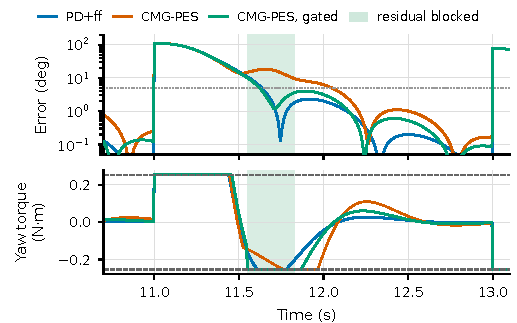
\includegraphics[width=\linewidth]{figures/11_hardstep/x2_hardstep_gate_zoom.pdf}
\caption{X2 Hardstep, one step at $t=11$ s: attitude error (log axis, dotted line: $5^\circ$ band) and yaw torque against the box $\pm\ell_z$ (dashed). Shading marks where the gate blocks the residual. Ungated, the residual pulls the command off the box during braking; gated, it follows PD+ff into the box and leaves it later.}
\label{fig:hardstep}
\end{figure}

The gate does not make the residual beat the baseline here, and Fig.~\ref{fig:hardstep} shows why. The gated residual helps while braking ($0.25$--$0.75$ s after a step; $-0.13^\circ$ of the X2 $45$-s mean) but leaves a larger tail once the baseline has left its box ($+0.40^\circ$ over $0.75$--$1.5$ s), because the decoder still holds the slew-phase correction, with the $9.6$ rad/s corner of Sec.~\ref{sec:ablation}. During these severe hard steps the torque limit is reached primarily on the main maneuver axis; the gate strictly inhibits only opposing residual authority on that saturated axis. Any small lag-induced transient on adjacent, unsaturated axes is therefore allowed to decay under the PES dynamics, so the gated architecture recovers baseline parity without post-saturation overshoot or cross-axis torque chattering.


%Hardstep commands $63^\circ$--$111^\circ$ attitude changes every $2$ s, and $97$--$99\%$ of its mean error accumulates during slew. At $\rho=3$ the ungated residual degrades it by $17.0\%$ on X2 and, at $\beta=.5$, diverges on CF2. Because the reference is piecewise constant, the latched decoder behaves like the first-order filter \eqref{eq:constantbasis}; on a saturated axis this lag can only oppose $\bm u_0$. At $\beta=.5$ the gate \eqref{eq:gate} blocks the residual in $20.5\%$ (X2) and $15.5\%$ (CF2) of Hardstep samples and in at most $0.04\%$ elsewhere. It cuts the X2 loss from $17.0\%$ to $2.0\%$ and, noise-free, removes the CF2 divergence at $\beta=.5$.

%The gate restores near-parity but does not beat the baseline, because decoder lag can leave a settling tail on unsaturated axes, which saturation-conditioned gating cannot remove.

%%%%%%%%%%%%%%%%%%%%%%%%%%%%%%%%%%%%%%%%%%%%%%%%%%%%%%%%%%%%%%%%%
\section{Conclusions and Future Work}
\label{sec:conclusion}
%%%%%%%%%%%%%%%%%%%%%%%%%%%%%%%%%%%%%%%%%%%%%%%%%%%%%%%%%%%%%%%%%

Six continuous CMG units with an eighteen-parameter PES-adapted decoder form a bounded residual that augments a quaternion PD controller without changing its sensing, collective-thrust, allocation, or actuator interface. The interface bounds and exact zero-authority recovery hold independently of the learned weights, and the saturation-aware gate preserves both. In the numerical study, the gated residual lowers geometric-mean error against the bandwidth-tuned PD+feedforward baseline by $37.3\%$ on X2 and $22.4\%$ on CF2 noise-free, lowers burst-phase error under repeated torque disturbances, and keeps its benefit under sensor noise only where the baseline error exceeds the noise floor; the ablations identify online decoder adaptation and persistent activity (necessary, but not sufficient for low effort) as the principal mechanisms in the tested regime.

\noindent\textbf{Theoretical conclusions on implementation properties:} Proposition~\ref{prop:bounded} establishes (i)--(ii) bounded internal CMG/PES states within their prescribed operational domains and (iii) a plant-facing interface guarantee: the requested torque remains within the prescribed box $\mathcal U$ with a componentwise residual bound $|\delta_{k,i}|\le\beta\ell_i$, and the baseline command is recovered exactly when $\beta=0$, independently of the learned internal state. Remark~\ref{rem:pes} summarizes a fixed-feature PES contraction property that helps interpret activity-limited learning behavior, but does not imply closed-loop convergence.

Three limitations remain. On Hardstep the gate, designed for saturation-limited slews, restores near-parity for PD+ff but cannot remove the settling-tail lag of the latched decoder on an unsaturated axis, though other baselines can still gain on Hardstep under the same gate. On CF2 under noise, rotor-level saturation defeats a gate defined on the torque box and caps the usable authority at $\beta=.2$. And the noise-free geometric mean overstates the practical benefit, being dominated by missions whose baseline error is already near the noise floor.\looseness=-1

The present results are simulation based and do not provide a closed-loop stability certificate for the reported tracking experiments. Future work will add decoder-side lag compensation and an allocation-aware gate; evaluate under model mismatch; sweep the activity gain $G$ and conductance modulation $\chi$ more systematically; test retention with frozen weights and held-out missions; extend the wrapper, already confirmed across five classical control families in simulation, to 6-DOF; and validate the method on hardware.


%Six continuous CMG units with an eighteen-parameter PES-adapted decoder form a bounded residual that augments a quaternion PD controller without changing its sensing, thrust loop, allocation, or actuator interface. The interface bounds and exact zero-authority recovery hold independently of the learned weights, and the saturation-aware gate \eqref{eq:gate} preserves both. In simulation, the gated residual reduces geometric-mean error against a bandwidth-tuned PD+feedforward baseline by $37.3\%$ (X2) and $22.4\%$ (CF2) noise-free, lowers burst-phase error under repeated disturbances, and helps under sensor noise mainly where baseline error exceeds the noise floor; ablations identify online decoder adaptation and persistent activity as the main mechanisms.

%Limitations include Hardstep settling tails from decoder lag, CF2 rotor saturation under noise (usable authority capped at $\beta=.2$), and noise-free geometric means dominated by near-noise-floor missions. Future work will add decoder-side lag compensation and an allocation-aware gate; evaluate under model mismatch; compare against integral-action and matched-effort non-neural bases; and validate on hardware.

\bibliographystyle{IEEEtran}
\bibliography{references_ACC2027}
\end{document}
